\documentclass[aspectratio=169,11pt]{beamer}

% TEMA Y COLORES
\usetheme{Madrid}
\usecolortheme{whale}

\definecolor{primaryblue}{RGB}{0,102,153}
\definecolor{accentgreen}{RGB}{0,128,0}
\definecolor{accentorange}{RGB}{204,102,0}
\definecolor{darkgray}{RGB}{64,64,64}

\setbeamercolor{palette primary}{bg=primaryblue,fg=white}
\setbeamercolor{palette secondary}{bg=primaryblue!80,fg=white}
\setbeamercolor{palette tertiary}{bg=primaryblue!60,fg=white}
\setbeamercolor{structure}{fg=primaryblue}
\setbeamercolor{block title}{bg=primaryblue,fg=white}
\setbeamercolor{block body}{bg=primaryblue!10}
\setbeamercolor{block title example}{bg=accentgreen,fg=white}
\setbeamercolor{block body example}{bg=accentgreen!10}
\setbeamercolor{block title alerted}{bg=accentorange,fg=white}
\setbeamercolor{block body alerted}{bg=accentorange!10}

% PAQUETES
\usepackage[utf8]{inputenc}
\usepackage[T1]{fontenc}
\usepackage{amsmath,amssymb}
\usepackage{booktabs}
\usepackage{tikz}
\usepackage{pgfplots}
\usepackage{listings}
\usepackage{multicol}

\pgfplotsset{compat=1.17}

% CÓDIGO PYTHON
\lstdefinestyle{pythonstyle}{
    language=Python,
    basicstyle=\ttfamily\footnotesize,
    keywordstyle=\color{blue}\bfseries,
    stringstyle=\color{red},
    commentstyle=\color{accentgreen}\itshape,
    frame=single,
    breaklines=true,
    showstringspaces=false,
    backgroundcolor=\color{gray!10}
}

% NAVEGACIÓN Y PIE DE PÁGINA
\setbeamertemplate{navigation symbols}{}
\setbeamertemplate{footline}{
    \leavevmode%
    \hbox{%
        \begin{beamercolorbox}[wd=.333333\paperwidth,ht=2.25ex,dp=1ex,center]{author in head/foot}%
            \usebeamerfont{author in head/foot}Matemáticas Financieras
        \end{beamercolorbox}%
        \begin{beamercolorbox}[wd=.333333\paperwidth,ht=2.25ex,dp=1ex,center]{title in head/foot}%
            \usebeamerfont{title in head/foot}Sesión 6
        \end{beamercolorbox}%
        \begin{beamercolorbox}[wd=.333333\paperwidth,ht=2.25ex,dp=1ex,right]{date in head/foot}%
            \usebeamerfont{date in head/foot}\insertframenumber{} / \inserttotalframenumber\hspace*{2ex}
        \end{beamercolorbox}}%
    \vskip0pt%
}

\title[Sesión 6]{Anualidades Anticipadas y Perpetuidades}
\subtitle{Pagos al inicio y flujos infinitos}
\author{Matemáticas Financieras}
\institute{Valor del Dinero en el Tiempo}
\date{Semana 3 | Clase 2 | Duración: 1h 50min}

\begin{document}

% ===========================================
% SECCIÓN 1: PORTADA Y CONTENIDO
% ===========================================

\begin{frame}
    \titlepage
\end{frame}

\begin{frame}{Contenido de la Sesión}
    \tableofcontents
\end{frame}

% ===========================================
% SECCIÓN 2: INTRODUCCIÓN
% ===========================================
\section{Introducción}

\begin{frame}{Conexión con la Sesión Anterior}
    \begin{block}{Sesión 5: Anualidades Ordinarias}
        Aprendimos a calcular VP y VF de pagos realizados al \textbf{final} de cada período:
        \[
        PV = PMT \cdot \frac{1-(1+r)^{-n}}{r} \quad \text{y} \quad FV = PMT \cdot \frac{(1+r)^n - 1}{r}
        \]
    \end{block}

    \pause
    \vspace{0.3cm}

    \begin{alertblock}{Hoy exploramos dos extensiones}
        \begin{enumerate}
            \item \textbf{Anualidades anticipadas:} ¿Y si pagan al \textbf{inicio} de cada período?
            \item \textbf{Perpetuidades:} ¿Y si los pagos \textbf{nunca terminan}?
        \end{enumerate}
    \end{alertblock}
\end{frame}

\begin{frame}{Objetivos de Aprendizaje}
    Al finalizar esta sesión, serás capaz de:
    \begin{enumerate}
        \item Distinguir entre anualidades ordinarias y anticipadas
        \item Calcular VP y VF de anualidades anticipadas
        \item Entender y aplicar el concepto de perpetuidad
        \item Calcular el valor de perpetuidades simples y crecientes
        \item Aplicar estos conceptos a valuación de pensiones, rentas y dividendos
        \item Usar la HP 12C en modo BEG para anualidades anticipadas
    \end{enumerate}
\end{frame}

\begin{frame}{Motivación: Diferentes Momentos de Pago}
    \begin{columns}
        \begin{column}{0.48\textwidth}
            \textbf{Anualidad Ordinaria}

            \vspace{0.3cm}
            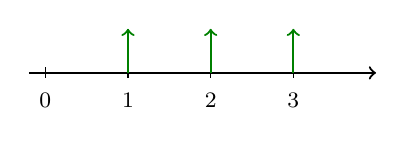
\begin{tikzpicture}[scale=0.7]
                \draw[thick, ->] (-0.3,0) -- (6,0);
                \foreach \x in {0, 1.5, 3, 4.5} {
                    \draw (\x,0.1) -- (\x,-0.1);
                }
                \node[below] at (0,-0.2) {\footnotesize 0};
                \node[below] at (1.5,-0.2) {\footnotesize 1};
                \node[below] at (3,-0.2) {\footnotesize 2};
                \node[below] at (4.5,-0.2) {\footnotesize 3};

                \draw[thick, ->, accentgreen] (1.5,0) -- (1.5,0.8);
                \draw[thick, ->, accentgreen] (3,0) -- (3,0.8);
                \draw[thick, ->, accentgreen] (4.5,0) -- (4.5,0.8);
            \end{tikzpicture}

            Pagos al \textbf{final}

            \textit{Ej: Préstamos, salarios}
        \end{column}

        \begin{column}{0.48\textwidth}
            \textbf{Anualidad Anticipada}

            \vspace{0.3cm}
            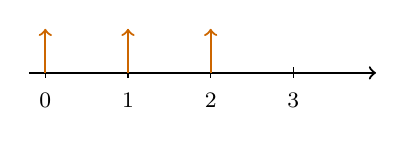
\begin{tikzpicture}[scale=0.7]
                \draw[thick, ->] (-0.3,0) -- (6,0);
                \foreach \x in {0, 1.5, 3, 4.5} {
                    \draw (\x,0.1) -- (\x,-0.1);
                }
                \node[below] at (0,-0.2) {\footnotesize 0};
                \node[below] at (1.5,-0.2) {\footnotesize 1};
                \node[below] at (3,-0.2) {\footnotesize 2};
                \node[below] at (4.5,-0.2) {\footnotesize 3};

                \draw[thick, ->, accentorange] (0,0) -- (0,0.8);
                \draw[thick, ->, accentorange] (1.5,0) -- (1.5,0.8);
                \draw[thick, ->, accentorange] (3,0) -- (3,0.8);
            \end{tikzpicture}

            Pagos al \textbf{inicio}

            \textit{Ej: Rentas, seguros}
        \end{column}
    \end{columns}

    \pause
    \vspace{0.5cm}

    \begin{exampleblock}{Pregunta Clave}
        Si ambas tienen los mismos pagos, ¿cuál vale más?

        \textbf{Respuesta:} La anticipada, porque cada pago llega un período antes.
    \end{exampleblock}
\end{frame}

% ===========================================
% SECCIÓN 3: ANUALIDADES ANTICIPADAS
% ===========================================
\section{Anualidades Anticipadas}

\begin{frame}{Comparación Visual: Ordinaria vs. Anticipada}
    \begin{center}
        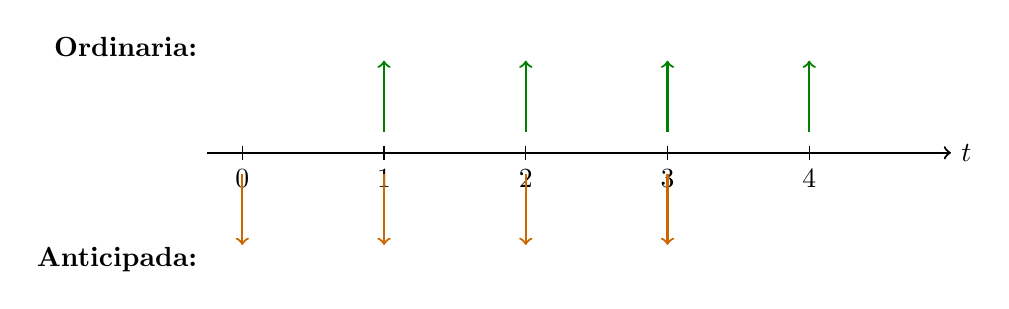
\begin{tikzpicture}[scale=0.9]
            % Línea de tiempo
            \draw[thick, ->] (-0.5,0) -- (10,0) node[right] {$t$};
            \foreach \x/\label in {0/0, 2/1, 4/2, 6/3, 8/4} {
                \draw (\x,0.1) -- (\x,-0.1) node[below] {\label};
            }

            % Ordinaria (arriba)
            \node[left] at (-0.5,1.5) {\textbf{Ordinaria:}};
            \foreach \x in {2, 4, 6, 8} {
                \draw[thick, ->, accentgreen] (\x,0.3) -- (\x,1.3);
            }

            % Anticipada (abajo)
            \node[left] at (-0.5,-1.5) {\textbf{Anticipada:}};
            \foreach \x in {0, 2, 4, 6} {
                \draw[thick, ->, accentorange] (\x,-0.3) -- (\x,-1.3);
            }
        \end{tikzpicture}
    \end{center}

    \pause
    \vspace{0.3cm}

    \textbf{Observación clave:}
    \begin{itemize}
        \item Ambas tienen 4 pagos de \$PMT
        \item La anticipada ``adelanta'' todos los pagos un período
        \item Cada pago de la anticipada tiene un período más para generar intereses (VF) o un período menos de descuento (VP)
    \end{itemize}
\end{frame}

\begin{frame}{Relación entre Ordinaria y Anticipada}
    \textbf{La anualidad anticipada es la ordinaria multiplicada por $(1+r)$:}

    \pause
    \vspace{0.3cm}

    \begin{block}{Valor Presente - Anualidad Anticipada}
        \[
        \boxed{PV_{\text{anticipada}} = PV_{\text{ordinaria}} \times (1+r) = PMT \cdot \frac{1-(1+r)^{-n}}{r} \cdot (1+r)}
        \]
    \end{block}

    \pause
    \vspace{0.3cm}

    \begin{block}{Valor Futuro - Anualidad Anticipada}
        \[
        \boxed{FV_{\text{anticipada}} = FV_{\text{ordinaria}} \times (1+r) = PMT \cdot \frac{(1+r)^n - 1}{r} \cdot (1+r)}
        \]
    \end{block}

    \pause
    \vspace{0.3cm}

    \begin{alertblock}{Intuición}
        Cada pago de la anticipada está ``un período adelante'', por lo que su valor es $(1+r)$ veces mayor.
    \end{alertblock}
\end{frame}

\begin{frame}{Derivación Alternativa del VP Anticipado}
    \textbf{Método directo:}

    \vspace{0.3cm}

    El VP de una anualidad anticipada es:
    \begin{align*}
        PV &= PMT + \frac{PMT}{(1+r)^1} + \frac{PMT}{(1+r)^2} + \cdots + \frac{PMT}{(1+r)^{n-1}}
    \end{align*}

    \pause
    \vspace{0.3cm}

    Comparando con la ordinaria que tiene pagos en períodos 1 a $n$:
    \begin{align*}
        PV_{\text{ord}} &= \frac{PMT}{(1+r)^1} + \frac{PMT}{(1+r)^2} + \cdots + \frac{PMT}{(1+r)^{n}}
    \end{align*}

    \pause
    \vspace{0.3cm}

    La anticipada tiene:
    \begin{itemize}
        \item Un pago extra en $t=0$ (sin descuento): $+PMT$
        \item Pero no tiene el pago en $t=n$: $-PMT/(1+r)^n$
    \end{itemize}
\end{frame}

\begin{frame}{Ejemplo: Renta de Departamento}
    \begin{block}{Problema}
        Rentas un departamento por \$15,000 mensuales, pagando al inicio de cada mes. Si el contrato es por 12 meses y la tasa es 1\% mensual, ¿cuál es el valor presente del contrato?
    \end{block}

    \pause
    \vspace{0.3cm}

    \textbf{Solución (método del factor):}
    \begin{align*}
        PV_{\text{ord}} &= 15,000 \cdot \frac{1-(1.01)^{-12}}{0.01} = 15,000 \times 11.2551 = \$168,826 \\[0.3cm]
        PV_{\text{ant}} &= PV_{\text{ord}} \times (1.01) = 168,826 \times 1.01 = \$170,514
    \end{align*}

    \pause
    \vspace{0.3cm}

    \textbf{Diferencia:} \$170,514 - \$168,826 = \$1,688

    Esto equivale a 1\% de \$168,826.
\end{frame}

% ===========================================
% SECCIÓN 4: PERPETUIDADES
% ===========================================
\section{Perpetuidades}

\begin{frame}{¿Qué es una Perpetuidad?}
    \begin{block}{Definición}
        Una \textbf{perpetuidad} es una anualidad que continúa \textbf{indefinidamente}; es decir, los pagos nunca terminan ($n \to \infty$).
    \end{block}

    \pause
    \vspace{0.3cm}

    \textbf{¿Existe en la práctica?}
    \begin{itemize}
        \item \textbf{Consols británicos:} Bonos emitidos por el gobierno británico que pagan cupones perpetuos (algunos desde el siglo XVIII)
        \item \textbf{Acciones preferentes:} Dividendos fijos sin fecha de vencimiento
        \item \textbf{Dotaciones universitarias:} Fondos que generan ingresos perpetuos
        \item \textbf{Aproximación:} Cualquier flujo de muy largo plazo (50+ años) puede modelarse como perpetuidad
    \end{itemize}
\end{frame}

\begin{frame}{Derivación del VP de una Perpetuidad}
    Partimos de la fórmula de anualidad ordinaria:
    \[
    PV = PMT \cdot \frac{1-(1+r)^{-n}}{r}
    \]

    \pause
    \vspace{0.3cm}

    Cuando $n \to \infty$:
    \begin{itemize}
        \item $(1+r)^{-n} \to 0$ (para $r > 0$)
    \end{itemize}

    \pause
    \vspace{0.3cm}

    Por lo tanto:
    \begin{align*}
        PV = PMT \cdot \frac{1 - 0}{r} = \frac{PMT}{r}
    \end{align*}

    \pause
    \begin{block}{Valor Presente de una Perpetuidad Simple}
        \[
        \boxed{PV = \frac{PMT}{r}}
        \]
    \end{block}
\end{frame}

\begin{frame}{Intuición de la Perpetuidad}
    \begin{exampleblock}{Interpretación Financiera}
        Si inviertes un capital $PV$ a tasa $r$, los intereses anuales son:
        \[
        \text{Intereses} = PV \times r
        \]

        Si solo retiras los intereses cada año, el capital permanece intacto.
        Por lo tanto, puedes retirar $PMT = PV \times r$ \textbf{para siempre}.
    \end{exampleblock}

    \pause
    \vspace{0.3cm}

    \textbf{Despejando:}
    \[
    PV = \frac{PMT}{r}
    \]

    \pause
    \vspace{0.3cm}

    \begin{alertblock}{Ejemplo}
        ¿Cuánto necesitas invertir al 5\% para recibir \$50,000 anuales perpetuos?

        $PV = 50,000 / 0.05 = \$1,000,000$
    \end{alertblock}
\end{frame}

\begin{frame}{Perpetuidad Creciente}
    \begin{block}{Definición}
        Una \textbf{perpetuidad creciente} es aquella donde los pagos crecen a una tasa constante $g$ cada período.
    \end{block}

    \pause
    \vspace{0.3cm}

    \textbf{Flujos:}
    \begin{itemize}
        \item Período 1: $PMT$
        \item Período 2: $PMT(1+g)$
        \item Período 3: $PMT(1+g)^2$
        \item Y así sucesivamente...
    \end{itemize}

    \pause
    \vspace{0.3cm}

    \begin{block}{Valor Presente de Perpetuidad Creciente (Modelo de Gordon)}
        \[
        \boxed{PV = \frac{PMT}{r - g}} \quad \text{donde } r > g
        \]
    \end{block}

    \pause
    \begin{alertblock}{Condición crítica}
        La tasa de descuento debe ser mayor que la tasa de crecimiento ($r > g$), de lo contrario el VP es infinito.
    \end{alertblock}
\end{frame}

\begin{frame}{Derivación de la Perpetuidad Creciente}
    \textbf{Serie de flujos:}
    \begin{align*}
        PV &= \frac{PMT}{1+r} + \frac{PMT(1+g)}{(1+r)^2} + \frac{PMT(1+g)^2}{(1+r)^3} + \cdots
    \end{align*}

    \pause
    Factorizando:
    \begin{align*}
        PV &= \frac{PMT}{1+r} \left[ 1 + \frac{1+g}{1+r} + \left(\frac{1+g}{1+r}\right)^2 + \cdots \right]
    \end{align*}

    \pause
    Si $r > g$, entonces $\frac{1+g}{1+r} < 1$ y la serie geométrica converge:
    \begin{align*}
        PV &= \frac{PMT}{1+r} \cdot \frac{1}{1 - \frac{1+g}{1+r}} = \frac{PMT}{1+r} \cdot \frac{1+r}{r-g} = \frac{PMT}{r-g}
    \end{align*}
\end{frame}

\begin{frame}{Ejemplo: Valuación de Acciones (Modelo de Gordon)}
    \begin{block}{Problema}
        Una acción paga un dividendo de \$5 por acción. Se espera que los dividendos crezcan 3\% anual perpetuamente. Si la tasa requerida es 10\%, ¿cuál es el precio justo de la acción?
    \end{block}

    \pause
    \vspace{0.3cm}

    \textbf{Nota:} El primer dividendo $D_1$ será dentro de un año: $D_1 = 5$

    \pause
    \textbf{Solución:}
    \begin{align*}
        P_0 &= \frac{D_1}{r - g} = \frac{5}{0.10 - 0.03} = \frac{5}{0.07} = \$71.43
    \end{align*}

    \pause
    \vspace{0.3cm}

    \begin{exampleblock}{Interpretación}
        Si compras la acción a \$71.43, obtendrás un rendimiento del 10\% anual (considerando dividendos + apreciación).
    \end{exampleblock}
\end{frame}

\begin{frame}{Sensibilidad del Modelo de Gordon}
    \textbf{¿Qué pasa si cambia la tasa de crecimiento?}

    \vspace{0.3cm}

    \begin{center}
    \begin{tabular}{@{}ccc@{}}
        \toprule
        $g$ & $r - g$ & $P_0 = D_1/(r-g)$ \\
        \midrule
        1\% & 9\% & \$55.56 \\
        2\% & 8\% & \$62.50 \\
        3\% & 7\% & \$71.43 \\
        4\% & 6\% & \$83.33 \\
        5\% & 5\% & \$100.00 \\
        \bottomrule
    \end{tabular}
    \end{center}

    \pause
    \vspace{0.3cm}

    \begin{alertblock}{Observación importante}
        El precio es muy sensible a pequeños cambios en $g$. Esta es una debilidad del modelo: pequeños errores en la estimación de $g$ generan grandes errores en la valuación.
    \end{alertblock}
\end{frame}

% ===========================================
% SECCIÓN 5: INTERPRETACIÓN VISUAL
% ===========================================
\section{Interpretación Visual}

\begin{frame}{Convergencia de Anualidad a Perpetuidad}
    \begin{center}
        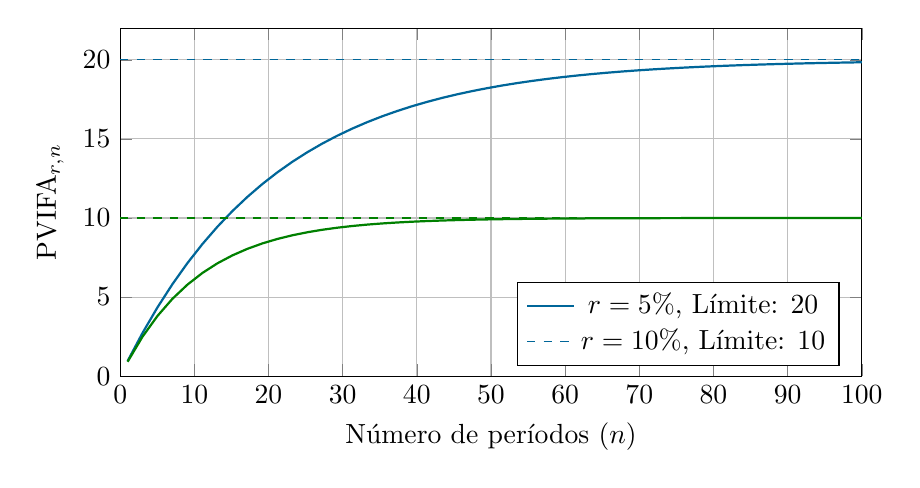
\begin{tikzpicture}
            \begin{axis}[
                xlabel={Número de períodos ($n$)},
                ylabel={PVIFA$_{r,n}$},
                xmin=0, xmax=100,
                ymin=0, ymax=22,
                grid=major,
                width=11cm,
                height=6cm,
                legend pos=south east
            ]
            % PVIFA al 5%
            \addplot[color=primaryblue, thick, domain=1:100, samples=50] {(1-(1.05)^(-x))/0.05};
            \addlegendentry{$r = 5\%$, Límite: 20}
            % Límite perpetuidad 5%
            \addplot[color=primaryblue, dashed, domain=0:100] {20};

            % PVIFA al 10%
            \addplot[color=accentgreen, thick, domain=1:100, samples=50] {(1-(1.10)^(-x))/0.10};
            \addlegendentry{$r = 10\%$, Límite: 10}
            % Límite perpetuidad 10%
            \addplot[color=accentgreen, dashed, domain=0:100] {10};
            \end{axis}
        \end{tikzpicture}
    \end{center}

    El PVIFA converge al límite $1/r$ (perpetuidad).
\end{frame}

\begin{frame}{Perpetuidad Simple vs. Creciente}
    \begin{center}
        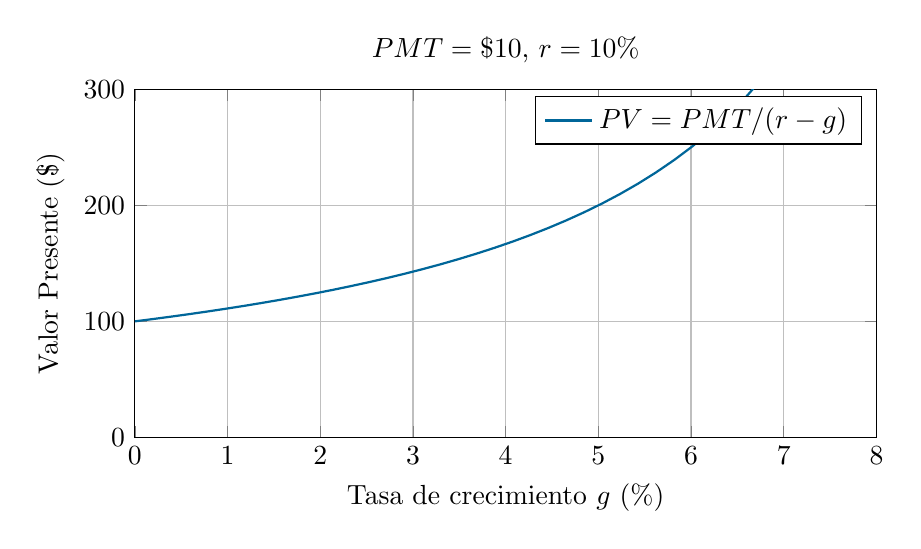
\begin{tikzpicture}
            \begin{axis}[
                xlabel={Tasa de crecimiento $g$ (\%)},
                ylabel={Valor Presente (\$)},
                xmin=0, xmax=8,
                ymin=0, ymax=300,
                grid=major,
                width=11cm,
                height=6cm,
                title={$PMT = \$10$, $r = 10\%$}
            ]
            % Perpetuidad creciente
            \addplot[color=primaryblue, thick, domain=0:9.5, samples=50] {10/(0.10 - x/100)};
            \addlegendentry{$PV = PMT/(r-g)$}
            % Línea vertical en r=g
            \addplot[color=red, dashed] coordinates {(10, 0) (10, 300)};
            \end{axis}
        \end{tikzpicture}
    \end{center}

    El valor explota cuando $g \to r$.
\end{frame}

% ===========================================
% SECCIÓN 6: TRUCOS DE ESTIMACIÓN
% ===========================================
\section{Trucos de Estimación Mental}

\begin{frame}{Perpetuidad: Múltiplos Rápidos}
    \begin{alertblock}{Regla del Múltiplo}
        El VP de una perpetuidad es el pago multiplicado por $1/r$:
        \[
        PV = PMT \times \text{Múltiplo}
        \]
    \end{alertblock}

    \pause
    \vspace{0.3cm}

    \begin{center}
    \begin{tabular}{@{}cc@{}}
        \toprule
        \textbf{Tasa} & \textbf{Múltiplo} \\
        \midrule
        5\% & 20x \\
        8\% & 12.5x \\
        10\% & 10x \\
        12.5\% & 8x \\
        20\% & 5x \\
        \bottomrule
    \end{tabular}
    \end{center}

    \pause
    \vspace{0.3cm}

    \begin{exampleblock}{Ejemplo}
        Pensión de \$30,000 anuales, tasa 10\%:

        $PV \approx 30,000 \times 10 = \$300,000$
    \end{exampleblock}
\end{frame}

\begin{frame}{Anticipada: Factor de Ajuste}
    \begin{alertblock}{Regla del $(1+r)$}
        Para convertir cualquier cálculo de ordinaria a anticipada:
        \[
        \text{Valor anticipada} = \text{Valor ordinaria} \times (1+r)
        \]
    \end{alertblock}

    \pause
    \vspace{0.5cm}

    \textbf{Ejemplo mental:}

    Si una anualidad ordinaria vale \$100,000 al 8\%:

    La misma anualidad anticipada vale: $100,000 \times 1.08 = \$108,000$

    \pause
    \vspace{0.3cm}

    \begin{exampleblock}{Aproximación adicional}
        Para tasas pequeñas ($r < 10\%$), el ajuste es aproximadamente $+r\%$ del valor ordinario.

        Ej: Al 5\%, la anticipada vale $\approx$ 5\% más que la ordinaria.
    \end{exampleblock}
\end{frame}

\begin{frame}{Perpetuidad Creciente: Estimación}
    \begin{alertblock}{Impacto del Crecimiento}
        Cada punto porcentual de crecimiento aumenta el múltiplo significativamente:
    \end{alertblock}

    \vspace{0.3cm}

    \begin{center}
    \begin{tabular}{@{}ccc@{}}
        \toprule
        $g$ & $r - g$ (si $r=10\%$) & Múltiplo \\
        \midrule
        0\% & 10\% & 10x \\
        2\% & 8\% & 12.5x \\
        4\% & 6\% & 16.7x \\
        5\% & 5\% & 20x \\
        \bottomrule
    \end{tabular}
    \end{center}

    \pause
    \vspace{0.3cm}

    \textbf{Regla práctica:}

    Si $g$ es la mitad de $r$, el múltiplo se duplica.

    (De 10x a 20x cuando $g$ pasa de 0\% a 5\%, con $r = 10\%$)
\end{frame}

% ===========================================
% SECCIÓN 7: HP 12C
% ===========================================
\section{Calculadora HP 12C}

\begin{frame}{HP 12C: Modo BEGIN para Anticipadas}
    \begin{center}
    \begin{tabular}{@{}cl@{}}
        \toprule
        \textbf{Teclas} & \textbf{Función} \\
        \midrule
        \texttt{g END} & Modo anualidad ordinaria (pagos al final) \\
        \texttt{g BEG} & Modo anualidad anticipada (pagos al inicio) \\
        \bottomrule
    \end{tabular}
    \end{center}

    \pause
    \vspace{0.3cm}

    \begin{alertblock}{Indicador visual}
        Cuando está en modo BEG, aparece ``BEGIN'' en la parte inferior del display.

        Si no aparece, está en modo END (ordinaria).
    \end{alertblock}

    \pause
    \vspace{0.3cm}

    \begin{exampleblock}{Consejo}
        Siempre verifica en qué modo estás antes de calcular. El modo persiste hasta que lo cambies.
    \end{exampleblock}
\end{frame}

\begin{frame}{HP 12C: Ejemplo - Renta Anticipada}
    \begin{block}{Problema}
        Renta mensual de \$12,000, contrato de 24 meses, 0.8\% mensual. ¿Cuál es el VP si se paga al inicio de cada mes?
    \end{block}

    \pause
    \vspace{0.3cm}

    \begin{center}
    \begin{tabular}{@{}lll@{}}
        \toprule
        \textbf{Teclas} & \textbf{Display} & \textbf{Descripción} \\
        \midrule
        \texttt{f CLX} & 0.00 & Limpiar \\
        \texttt{g BEG} & BEGIN & Modo anticipada \\
        \texttt{12000 PMT} & 12,000.00 & Pago mensual \\
        \texttt{24 n} & 24.00 & 24 meses \\
        \texttt{0.8 i} & 0.80 & 0.8\% mensual \\
        \texttt{0 FV} & 0.00 & Sin valor final \\
        \texttt{PV} & \textbf{-264,982.78} & VP anticipada \\
        \bottomrule
    \end{tabular}
    \end{center}

    \pause
    \textbf{Comparación:} En modo END sería \$262,887.72 (1.8\% menos).
\end{frame}

\begin{frame}{HP 12C: Ejemplo - Fondo de Retiro Anticipado}
    \begin{block}{Problema}
        Depositas \$5,000 mensuales al inicio de cada mes por 20 años al 0.6\% mensual. ¿Cuánto acumulas?
    \end{block}

    \pause
    \vspace{0.3cm}

    \begin{center}
    \begin{tabular}{@{}lll@{}}
        \toprule
        \textbf{Teclas} & \textbf{Display} & \textbf{Descripción} \\
        \midrule
        \texttt{f CLX} & 0.00 & Limpiar \\
        \texttt{g BEG} & BEGIN & Modo anticipada \\
        \texttt{5000 CHS PMT} & -5,000.00 & Depósito mensual \\
        \texttt{240 n} & 240.00 & 240 meses \\
        \texttt{0.6 i} & 0.60 & 0.6\% mensual \\
        \texttt{0 PV} & 0.00 & Sin inversión inicial \\
        \texttt{FV} & \textbf{2,357,892.50} & Valor futuro \\
        \bottomrule
    \end{tabular}
    \end{center}

    \pause
    Depositaste: $5,000 \times 240 = \$1,200,000$. Ganaste \$1,157,892 en intereses.
\end{frame}

\begin{frame}{HP 12C: Perpetuidades (Cálculo Manual)}
    La HP 12C no tiene función de perpetuidad, pero es fácil calcular:

    \pause
    \vspace{0.3cm}

    \begin{block}{Perpetuidad Simple: $PV = PMT/r$}
        \begin{center}
        \begin{tabular}{@{}lll@{}}
            \textbf{Teclas} & \textbf{Display} & \textbf{Descripción} \\
            \midrule
            \texttt{50000 ENTER} & 50,000 & PMT \\
            \texttt{0.08 $\div$} & \textbf{625,000} & PV = PMT/r \\
        \end{tabular}
        \end{center}
    \end{block}

    \pause
    \vspace{0.3cm}

    \begin{block}{Perpetuidad Creciente: $PV = PMT/(r-g)$}
        \begin{center}
        \begin{tabular}{@{}lll@{}}
            \textbf{Teclas} & \textbf{Display} & \textbf{Descripción} \\
            \midrule
            \texttt{50000 ENTER} & 50,000 & PMT \\
            \texttt{0.08 ENTER 0.03 -} & 0.05 & $r - g$ \\
            \texttt{$\div$} & \textbf{1,000,000} & PV \\
        \end{tabular}
        \end{center}
    \end{block}
\end{frame}

% ===========================================
% SECCIÓN 8: EJERCICIOS PRÁCTICOS
% ===========================================
\section{Ejercicios Prácticos}

\begin{frame}{Ejercicio 1: Arrendamiento}
    \begin{block}{Problema}
        Un arrendamiento requiere pagos de \$8,000 al inicio de cada mes por 36 meses. Si la tasa es 1.2\% mensual, ¿cuál es el valor presente del arrendamiento?
    \end{block}

    \pause
    \vspace{0.3cm}

    \textbf{Solución:}

    Primero, VP ordinario:
    \begin{align*}
        PV_{\text{ord}} = 8,000 \cdot \frac{1-(1.012)^{-36}}{0.012} = 8,000 \times 28.8473 = \$230,778
    \end{align*}

    \pause
    Luego, ajustar a anticipada:
    \begin{align*}
        PV_{\text{ant}} = 230,778 \times 1.012 = \$233,547
    \end{align*}

    \pause
    \textbf{Diferencia:} La anticipada vale \$2,769 más (1.2\% más).
\end{frame}

\begin{frame}{Ejercicio 2: Perpetuidad Simple}
    \begin{block}{Problema}
        Una fundación quiere establecer una beca perpetua de \$100,000 anuales. Si la tasa de rendimiento esperada es 6\%, ¿cuánto debe donar hoy?
    \end{block}

    \pause
    \vspace{0.3cm}

    \textbf{Solución:}
    \begin{align*}
        PV = \frac{PMT}{r} = \frac{100,000}{0.06} = \$1,666,667
    \end{align*}

    \pause
    \vspace{0.3cm}

    \begin{exampleblock}{Verificación}
        Con \$1,666,667 al 6\%:

        Intereses anuales = $1,666,667 \times 0.06 = \$100,000$ \checkmark

        El capital permanece intacto.
    \end{exampleblock}
\end{frame}

\begin{frame}{Ejercicio 3: Perpetuidad Creciente}
    \begin{block}{Problema}
        Un bono perpetuo paga un cupón de \$80 el próximo año, y los cupones crecerán 2\% anual indefinidamente. Si la tasa requerida es 9\%, ¿cuál es el precio del bono?
    \end{block}

    \pause
    \vspace{0.3cm}

    \textbf{Solución:}
    \begin{align*}
        PV = \frac{C_1}{r - g} = \frac{80}{0.09 - 0.02} = \frac{80}{0.07} = \$1,142.86
    \end{align*}

    \pause
    \vspace{0.3cm}

    \textbf{Comparación con perpetuidad simple:}

    Sin crecimiento: $PV = 80/0.09 = \$888.89$

    El crecimiento del 2\% agrega \$253.97 de valor (29\% más).
\end{frame}

\begin{frame}{Ejercicio 4: Valuación de Empresa}
    \begin{block}{Problema}
        Una empresa genera flujos de caja de \$500,000 anuales, creciendo 4\% perpetuamente. Si el costo de capital es 12\%, ¿cuál es el valor de la empresa?
    \end{block}

    \pause
    \vspace{0.3cm}

    \textbf{Solución (Modelo de Gordon para empresas):}
    \begin{align*}
        V_0 = \frac{CF_1}{r - g} = \frac{500,000}{0.12 - 0.04} = \frac{500,000}{0.08} = \$6,250,000
    \end{align*}

    \pause
    \vspace{0.3cm}

    \begin{alertblock}{Sensibilidad}
        Si $g$ fuera 5\%: $V = 500,000/0.07 = \$7,142,857$ (+14\%)

        Si $g$ fuera 3\%: $V = 500,000/0.09 = \$5,555,556$ (-11\%)
    \end{alertblock}
\end{frame}

\begin{frame}{Ejercicio 5: Pensión Anticipada}
    \begin{block}{Problema}
        Un plan de pensión pagará \$20,000 mensuales al inicio de cada mes por 25 años. Si la tasa es 0.5\% mensual, ¿cuál es el valor actual de la pensión?
    \end{block}

    \pause
    \vspace{0.3cm}

    \textbf{Datos:} $n = 300$ meses, $r = 0.5\%$

    \textbf{Solución:}
    \begin{align*}
        PV_{\text{ord}} &= 20,000 \cdot \frac{1-(1.005)^{-300}}{0.005} = 20,000 \times 155.207 = \$3,104,140 \\[0.2cm]
        PV_{\text{ant}} &= 3,104,140 \times 1.005 = \$3,119,661
    \end{align*}

    \pause
    La pensión anticipada vale \$3,119,661.
\end{frame}

% ===========================================
% SECCIÓN 9: PYTHON
% ===========================================
\section{Python con numpy-financial}

\begin{frame}[fragile]{Python: Anualidades Anticipadas}
    \begin{lstlisting}[style=pythonstyle]
import numpy_financial as npf

# Anualidad anticipada con numpy-financial
# Usar parametro 'when' = 'begin' (o 1)

pmt = 12000
n = 24
r = 0.008

# Anualidad ordinaria
pv_ord = npf.pv(rate=r, nper=n, pmt=pmt, fv=0, when='end')
print(f"VP Ordinaria: ${-pv_ord:,.2f}")

# Anualidad anticipada
pv_ant = npf.pv(rate=r, nper=n, pmt=pmt, fv=0, when='begin')
print(f"VP Anticipada: ${-pv_ant:,.2f}")

# Verificacion: diferencia es factor (1+r)
print(f"Ratio: {-pv_ant/-pv_ord:.4f}")
print(f"(1+r) = {1+r:.4f}")
    \end{lstlisting}
\end{frame}

\begin{frame}[fragile]{Python: Perpetuidades}
    \begin{lstlisting}[style=pythonstyle]
def perpetuidad_simple(pmt, r):
    """Valor presente de perpetuidad simple."""
    return pmt / r

def perpetuidad_creciente(pmt, r, g):
    """Valor presente de perpetuidad creciente (Gordon)."""
    if r <= g:
        raise ValueError("r debe ser mayor que g")
    return pmt / (r - g)

# Ejemplos
print("Perpetuidad Simple:")
print(f"  $50,000/año al 8%: ${perpetuidad_simple(50000, 0.08):,.2f}")

print("\nPerpetuidad Creciente:")
print(f"  $50,000 inicial, g=3%, r=8%: ${perpetuidad_creciente(50000, 0.08, 0.03):,.2f}")

# Sensibilidad
print("\nAnalisis de sensibilidad (PMT=$50,000, r=8%):")
for g in [0.01, 0.02, 0.03, 0.04, 0.05]:
    pv = perpetuidad_creciente(50000, 0.08, g)
    print(f"  g={g*100:.0f}%: ${pv:,.2f}")
    \end{lstlisting}
\end{frame}

\begin{frame}[fragile]{Python: Gráfica Comparativa}
    \begin{lstlisting}[style=pythonstyle]
import matplotlib.pyplot as plt
import numpy as np

pmt = 10000
r = 0.10
periodos = np.arange(1, 101)

# PVIFA ordinaria
pvifa_ord = [(1-(1+r)**(-n))/r for n in periodos]

# PVIFA anticipada
pvifa_ant = [pv * (1+r) for pv in pvifa_ord]

# Perpetuidad
perp = 1/r

plt.figure(figsize=(10, 6))
plt.plot(periodos, pvifa_ord, 'b-', label='Ordinaria')
plt.plot(periodos, pvifa_ant, 'g-', label='Anticipada')
plt.axhline(y=perp, color='r', linestyle='--', label=f'Perpetuidad: {perp}')
plt.xlabel('Numero de periodos')
plt.ylabel('Factor PVIFA')
plt.title('Convergencia a Perpetuidad')
plt.legend()
plt.grid(True)
    \end{lstlisting}
\end{frame}

% ===========================================
% SECCIÓN 10: RESUMEN Y TAREA
% ===========================================
\section{Resumen y Tarea}

\begin{frame}{Resumen de Fórmulas}
    \begin{columns}
        \begin{column}{0.5\textwidth}
            \textbf{Anualidad Anticipada}
            \begin{align*}
                PV_{\text{ant}} &= PV_{\text{ord}} \times (1+r) \\[0.3cm]
                FV_{\text{ant}} &= FV_{\text{ord}} \times (1+r)
            \end{align*}

            \vspace{0.3cm}

            \textbf{Perpetuidad Simple}
            \[
            PV = \frac{PMT}{r}
            \]
        \end{column}

        \begin{column}{0.5\textwidth}
            \textbf{Perpetuidad Creciente}
            \[
            PV = \frac{PMT}{r - g} \quad (r > g)
            \]

            \vspace{0.5cm}

            \textbf{Múltiplos rápidos}
            \begin{align*}
                5\% &\to 20\times \\
                10\% &\to 10\times
            \end{align*}
        \end{column}
    \end{columns}
\end{frame}

\begin{frame}{Conceptos Clave}
    \begin{enumerate}
        \item \textbf{Anualidad anticipada}: pagos al inicio, vale $(1+r)$ más
        \item \textbf{Perpetuidad}: anualidad infinita, $PV = PMT/r$
        \item \textbf{Perpetuidad creciente}: considera crecimiento, $PV = PMT/(r-g)$
        \item El \textbf{Modelo de Gordon} es una perpetuidad creciente
        \item La perpetuidad es el límite de la anualidad cuando $n \to \infty$
        \item HP 12C: usar \texttt{g BEG} para anticipadas
        \item El valor es muy sensible a $g$ cuando $g$ se acerca a $r$
    \end{enumerate}
\end{frame}

\begin{frame}{Tarea para la Próxima Sesión}
    \begin{enumerate}
        \item \textbf{Ejercicios HP 12C:}
        \begin{itemize}
            \item VP de renta de \$18,000 mensual anticipada, 36 meses, 1\%
            \item VF de depósitos de \$2,000 al inicio del mes, 60 meses, 0.7\%
        \end{itemize}

        \vspace{0.3cm}

        \item \textbf{Perpetuidad:} ¿Cuánto debes invertir al 7\% para recibir \$80,000 anuales perpetuos?

        \vspace{0.3cm}

        \item \textbf{Modelo de Gordon:} Una acción pagará \$3 de dividendo el próximo año. Si los dividendos crecen 4\% y la tasa requerida es 11\%, ¿cuál es el precio?

        \vspace{0.3cm}

        \item \textbf{Python:} Grafica el valor de una perpetuidad creciente para $g$ variando de 0\% a 9\%, con $r = 10\%$ y $PMT = \$1,000$.
    \end{enumerate}
\end{frame}

% ===========================================
% CIERRE
% ===========================================

\begin{frame}
    \begin{center}
        \Huge \textcolor{primaryblue}{\textbf{¿Preguntas?}}

        \vspace{1cm}
        \Large Próxima Sesión:\\
        \textbf{Amortización de Préstamos}

        \vspace{0.5cm}
        \normalsize Semana 4, Clase 1
    \end{center}
\end{frame}

\end{document}
